\documentclass[24pt,margin=.9in,innermargin=-4.5in,blockverticalspace=0.3in]{tikzposter}
\geometry{paperwidth=42in,paperheight=30in}
 \renewcommand{\familydefault}{\sfdefault}
\usepackage[utf8]{inputenc}
\usepackage{amsmath}
\usepackage{amsfonts}
\usepackage{amsthm}
\usepackage{amssymb}
\usepackage{mathrsfs}
\usepackage{graphicx}
\usepackage{adjustbox}
\usepackage{enumitem}
\usepackage{amsfonts}
\newcommand{\indep}{{\bot\negthickspace\negthickspace\bot}}
\newcommand{\E}{{\rm I\kern-.3em E}}
\newcommand{\Var}{\text{Var}}
\newcommand{\V}{\text{V}}
\newcommand{\N}{\mathcal{N}}
\newcommand{\I}{\text{I}}
\newcommand{\Cov}{\text{Cov}}
\newcommand{\Cor}{\text{Cor}}
\renewcommand{\P}{\text{P}}
\newcommand{\doop}{\text{do}}
\newcommand{\bblue}[1]{\textbf{\textcolor{blue}{#1}}}
\newcommand{\bgreen}[1]{\textbf{\textcolor{olive}{#1}}}
\usepackage{emory-theme}
\newcommand\mydots{\hbox to 1em{.\hss.\hss.}}
\usepackage{tikz}
\usetikzlibrary{arrows,shapes.arrows,positioning,shapes}
\usepackage[round]{natbib}
\bibliographystyle{humannat-mod}
\renewcommand\refname{}
%\bibstyle{default}
%\usepackage[backend=biber,style=numeric]{biblatex}
%\addbibresource{FF_housing_assistance.bib}

% set theme parameters
\tikzposterlatexaffectionproofoff
\usetheme{EmoryTheme}
\usecolorstyle{EmoryStyle}

\title{\begin{minipage}[h]{2in}\end{minipage}\begin{minipage}[h]{38in}\centering \vspace{-.7in}Government assistance protects low-income families from eviction and rent nonpayment\end{minipage}\begin{minipage}[h]{2in}
\includegraphics[width = 2in]{figures/assistance_qr.png}\end{minipage}}
\author{\vspace{-1.2in} Ian Lundberg\textsuperscript{ab}, Sarah L. Gold\textsuperscript{b}, Louis Donnelly\textsuperscript{bc}, Jeanne Brooks-Gunn\textsuperscript{d}, and Sara S. McLanahan\textsuperscript{abcd}\\
\textsuperscript{a}Department of Sociology, \textsuperscript{b}Office of Population Research, \textsuperscript{a}Center for Research on Child Wellbeing, Princeton University\quad\textsuperscript{d}Teachers College and College of Physicians and Surgeons, Columbia University}

% begin document
\begin{document}

\maketitle
\centering
\begin{columns}
    \column{0.32}
    \block{The Affordable Housing Crisis Demands a Policy Response}{
        	Eviction is \bgreen{common}.
         \begin{itemize}
         \item 2 \% of rental households evicted in 2016 \citep{desmond2018}
         \item 15 \% of children born in large U.S. cities in 1998--2000 were evicted by age 15 \citep{lundberg2019}
         %\item XX missed rent payment.
         \end{itemize} \vskip .2in
        	Eviction is \bgreen{harmful}. Eviction leads to:
         \begin{itemize}
         \item More material hardship \citep{desmondkimbro2015}
         \item More residential instability \citep{desmond2015a}
         \end{itemize}
         Available evidence may inform policies to address these problems.
    }
    \block{Research Question}{
    	Does government assistance protect low-income families\\from \bblue{rent nonpayment} and \bblue{eviction}?
	\begin{center}
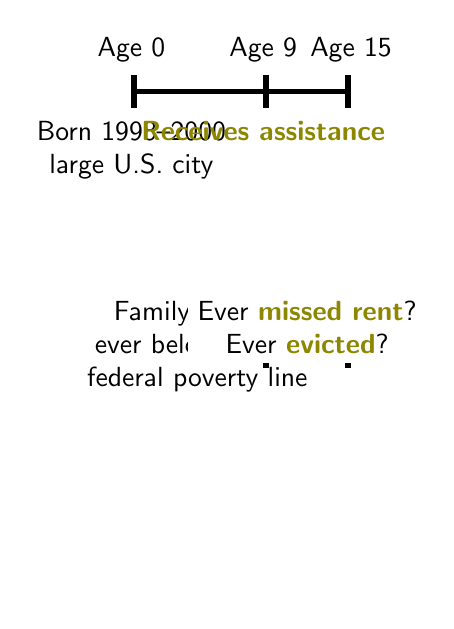
\begin{tikzpicture}[x = .23\textwidth, y = 1in]
\node at (-.13, -2.5) {};
\node at (1.125, 0) {};
\draw[|-, line width = 2pt] (0,0) -- (9/15,0);
\node[anchor = south, align=center, font = \normalsize] at (0,.1) {Age 0};
\draw[|-|, line width = 2pt] (9/15,0) -- (1,0);
\node[anchor = south, align=center, font = \normalsize] at (9/15,.1) {Age 9};
\node[anchor = south, align=center, font = \normalsize] at (1,.1) {Age 15};
\node[anchor = north,align=center, font = \normalsize] at (0,-.1) {Born 1998--2000\\large U.S. city};
\draw[|-, line width = 2pt] (0,-1.3) -- (9/15,-1.3);
\node[anchor = north,align=center, font = \normalsize, fill = white] at (4.5/15,-1) {Family income\\ever below 200 \%\\federal poverty line};
\node[anchor = north,align=center, font = \normalsize] at (9/15,-.1) {\bgreen{Receives assistance}};
\draw[|-|, line width = 2pt] (9/15,-1.3) -- (15/15,-1.3);
\node[anchor = north,align=center, font = \normalsize, fill = white] at (12/15,-1) {Ever \bgreen{missed rent}?\\Ever \bgreen{evicted}?};
\end{tikzpicture}
\end{center}\vspace{-.6in}
}
    \block{Data}{
    \bgreen{Fragile Families and Child Wellbeing Study}: Probability sample of 1998--2000 births in U.S. cities with populations over 200k \vskip .2in
    \begin{center}
    \begin{tabular}{p{.21\textwidth}p{.05\textwidth}}
    \textbf{Restriction} & \textbf{Families} \\
    \hline
    Full sample & 4,898 \\
    Resided with responding mother or father at age 9 & 3,512 \\
    Not residing in an owned home & 2,488 \\
    <200\% federal poverty line at some point & 2,305 \\
    Not missing treatment variable & 2,219 \\
    \hline
    \end{tabular} \vskip .2cm
    \end{center}\vskip .4in
    \begin{center}
    
\begin{tikzpicture}[x = 11.1in]
    \draw[fill = gray, draw = gray, rounded corners] (-.5,-1) rectangle (.5, 1);
    \node[white, font = {\bf\Large}] at (0,0) {References};
    \end{tikzpicture}
    \end{center}
    \begin{minipage}{.3\textwidth}
    \footnotesize
    \vspace{-.3in}
        \bibliography{FF_housing_assistance.bib}
        %\printbibliography[heading=none]
        \end{minipage}
    } 
    \column{0.36}
    \block{Descriptive Statistics}{
    \vspace{-.4in}
%Descriptive statistics for analytic sample ($N$ = 2,219). Missing values are imputed. All estimates are unweighted. Incomes are top-coded at five times the poverty line.
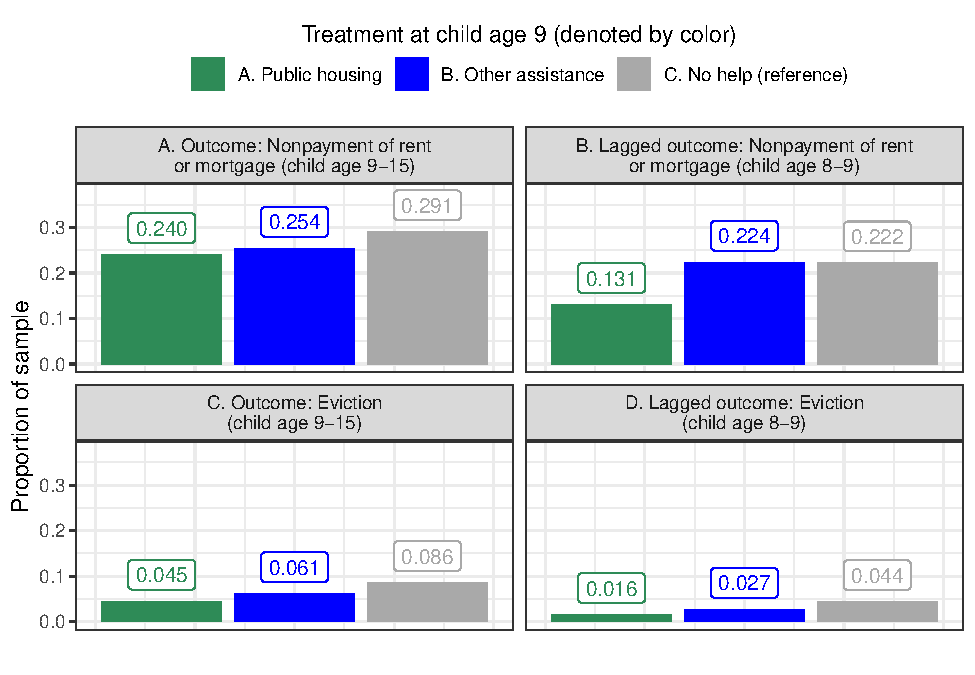
\includegraphics[width = .3\textwidth]{figures/descriptives_outcomes} \\
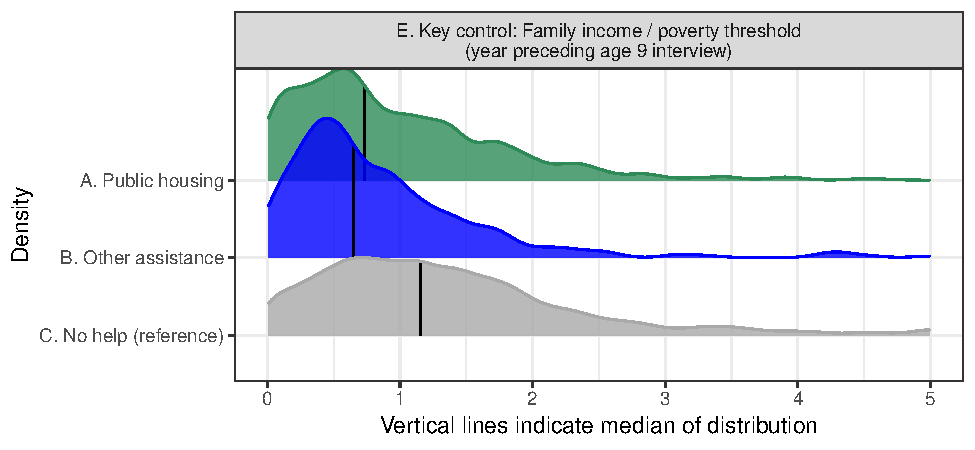
\includegraphics[width = .3\textwidth]{figures/descriptives_income}
}
    \block{Assumptions for Causal Inference}{
        \begin{center}
        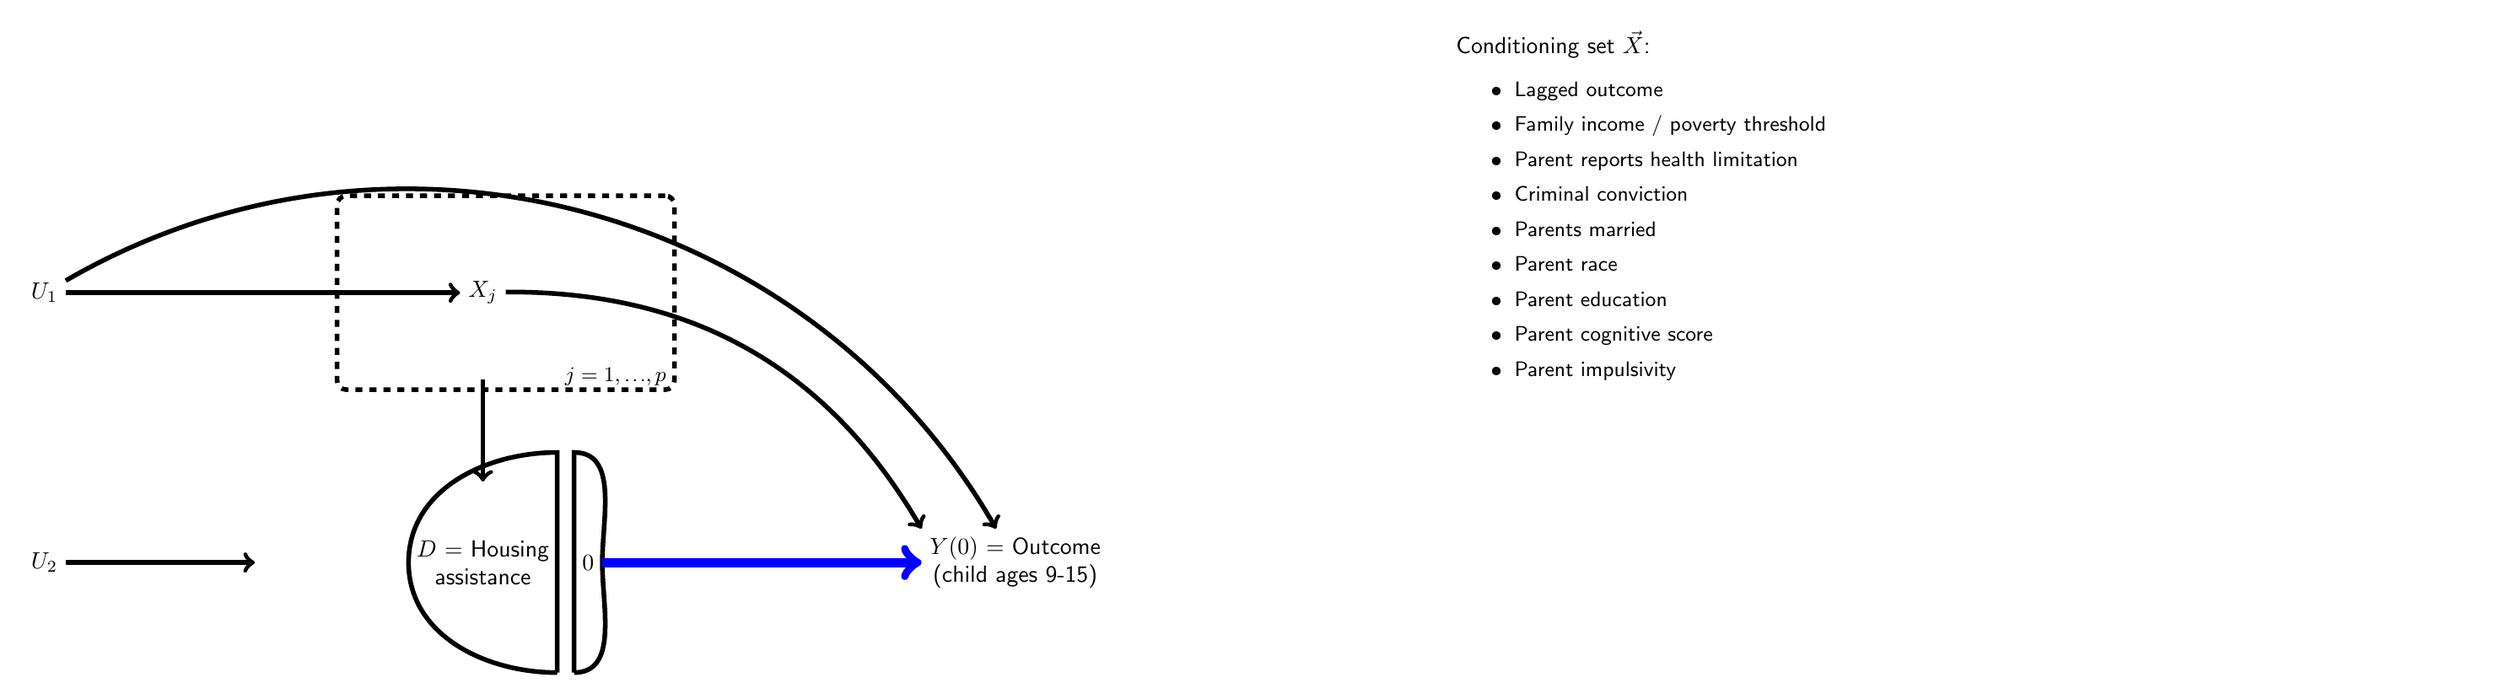
\begin{tikzpicture}[x = 2.6in, y = 1.6in]
	%\node[align = center] at (.5,2.5) {\textbf{a)} Effect is identified};
	\node[align = center] (xj) at (0,1) {$X_j$};
	\node[align = right, font = \small, shift = {(1in,-.6in)}, anchor = south east] at (xj.east) {$j = 1,\mydots,p$};
	\node[align = center, draw, line width = 2pt, rounded corners, dashed, minimum width = 2in, minimum height = 1.15in] at (xj.east) {};
	\node[align = center, minimum height = 1.3in] (d) at (0,0) {$D$ = Housing\\assistance};
	\node[right = .1in of d, align = center, anchor = west, minimum height = 1.3in] (d_fixed) {$0$};
	\draw[line width = 2pt] (d.south east) to[out = 180, in = 270] (d.west) to[out = 90, in = 180] (d.north east) -- (d.south east);
	\draw[line width = 2pt] (d_fixed.south west) to[out = 0, in = 270] (d_fixed.east) to[out = 90, in = 0] (d_fixed.north west) -- (d_fixed.south west);
	\node[align = center, anchor = west] (y) at (1,0) {$Y(0)$ = Outcome\\(child ages 9-15)};
	\node[align = center] (u2) at (-1,0) {$U_2$};
	\draw[->, line width = 2pt] (u2) -- (-.52,0);
	\node[align = center] (u1) at (-1,1) {$U_1$};
	\draw[->, line width = 2pt] (u1) to[bend left = 45] (y);
	%to[out = 60, in = 180] (0,1.5) to[out = 0, in = 90] (y);
	\draw[->, line width = 2pt] (u1) -- (xj);
	%\node[align = center, font = \footnotesize] (u1) at (0,2) {$U_1$};
	\draw[->, line width = 2pt] (0,.68) -- (0,.3);
	\draw[->, line width = 2pt] (xj) to[bend left] (y.north west);
	%\draw[->, thick] (u1) to[bend left] (y);
	%\draw[->, thick] (u1) -- (xj);
	\draw[->, line width = 4pt, blue] (d_fixed) -- (y);
	\node[anchor = north west] at (2.2,2) {\begin{minipage}{6in}
	Conditioning set $\vec{X}$: \vskip .1in
	\begin{small}
	\begin{itemize}
	\item Lagged outcome
	\item Family income / poverty threshold
	\item Parent reports health limitation
	\item Criminal conviction
	\item Parents married
	\item Parent race
	\item Parent education
	\item Parent cognitive score
	\item Parent impulsivity
	\end{itemize}\end{small}
	\end{minipage}};
	\end{tikzpicture}
	\end{center}
	\bgreen{Identification Assumption:} Within subgroups of $\vec{X}$, all dependence between housing assistance and the outcome arises from the causal effect. \vskip .2cm
	\bgreen{Estimation Assumption:} $\P(Y\mid \vec{X} = \vec{x}, D = d) = \vec{X}\beta_d$
    }
    \column{0.32}    
    \block{Results}{
    Nonpayment of rent or mortgage and eviction between child ages 9 and 15 are \bgreen{much less common} among those residing in public housing or receiving other assistance, compared with those receiving no assistance.\\
    If the required assumptions hold, this result can be interpreted causally: housing assistance protects against eviction and rent nonpayment. \vskip .6in
    	\begin{center}
        \begin{tikzpicture}[x = .65in,y = .62in]
\node at (0,0) {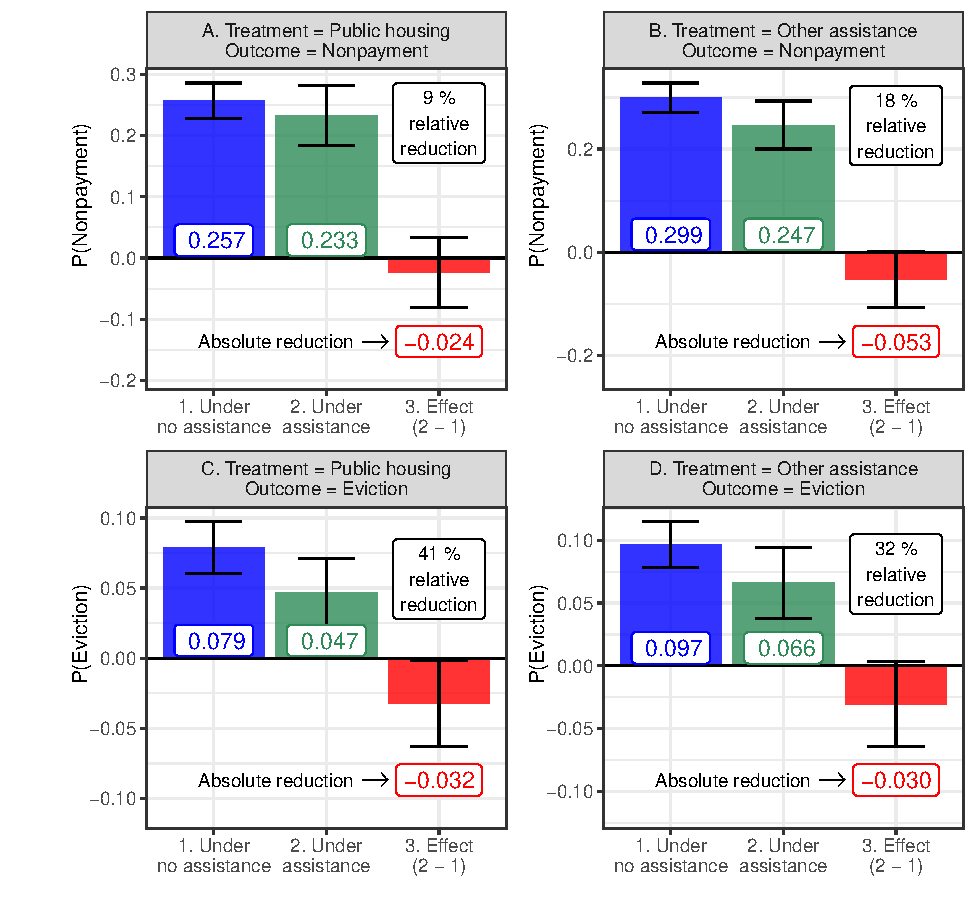
\includegraphics[width = .27\textwidth]{figures/effects_plot}};
\draw[rounded corners, thick, darkgray] (-8,0.1) rectangle (9,9);
\node[darkgray, font = \small] at (.5,8.25) {$F$-test jointly testing red effect bars: $p = .020$};
\draw[rounded corners, thick, darkgray] (-8,0.1) rectangle (9,-9);
\node[darkgray, font = \small] at (.5,-8.25) {$F$-test jointly testing red effect bars: $p = .003$};
\end{tikzpicture}
	\end{center}
    }
    
    \block{Discussion}{
        Government assistance may reduce eviction and rent nonpayment.
        \begin{enumerate}
        \item Future randomized evaluations may be worth the cost
        \item In the short term, government assistance may be a useful policy lever
        \end{enumerate}
    \begin{center} \vskip .6in
    
\begin{tikzpicture}[x = 11.1in]
    \draw[fill = gray, draw = gray, rounded corners] (-.5,-1) rectangle (.5, 1);
    \node[white, font = {\bf\Large}] at (0,0) {Acknowledgments};
    \end{tikzpicture} \vskip .2in
        \begin{minipage}{.28\textwidth}\footnotesize
        We thank Catherine Doren, the Stewart Lab, the Inequality Working Group, and a housing roundtable sponsored by the W.T. Grant Foundation at Princeton University for helpful comments on earlier drafts. Research reported in this publication was supported by the Robert Wood Johnson Foundation and by The Eunice Kennedy Shriver National Institute of Child Health \& Human Development of the National Institutes of Health under Award Number P2CHD047879. Funding for the Fragile Families Study was provided through Award Numbers R01HD36916, R01HD39135, and R01HD40421 and by a consortium of private foundations. The content is solely the responsibility of the authors and does not necessarily represent the official views of the National Institutes of Health.
        \end{minipage}
    \end{center}
    }
\end{columns}
\end{document}